\section{Experimental}
My role in this work was entirely on the analysis of the measurements and the development of the chemically-consistent model.\footnote{The experimental measurements were designed and conducted by Drs Tom Arnold, Andrew Jackson, Adrian Sanchez-Fernandez, and Prof. Karen Edler, with the assistance of Dr Richard Campbell.}
However, it is necessary to briefly discuss the materials and experimental methods used to enable a complete understanding of the context of the work.

\subsection{Materials}
%
\begin{marginfigure}
    \centering
    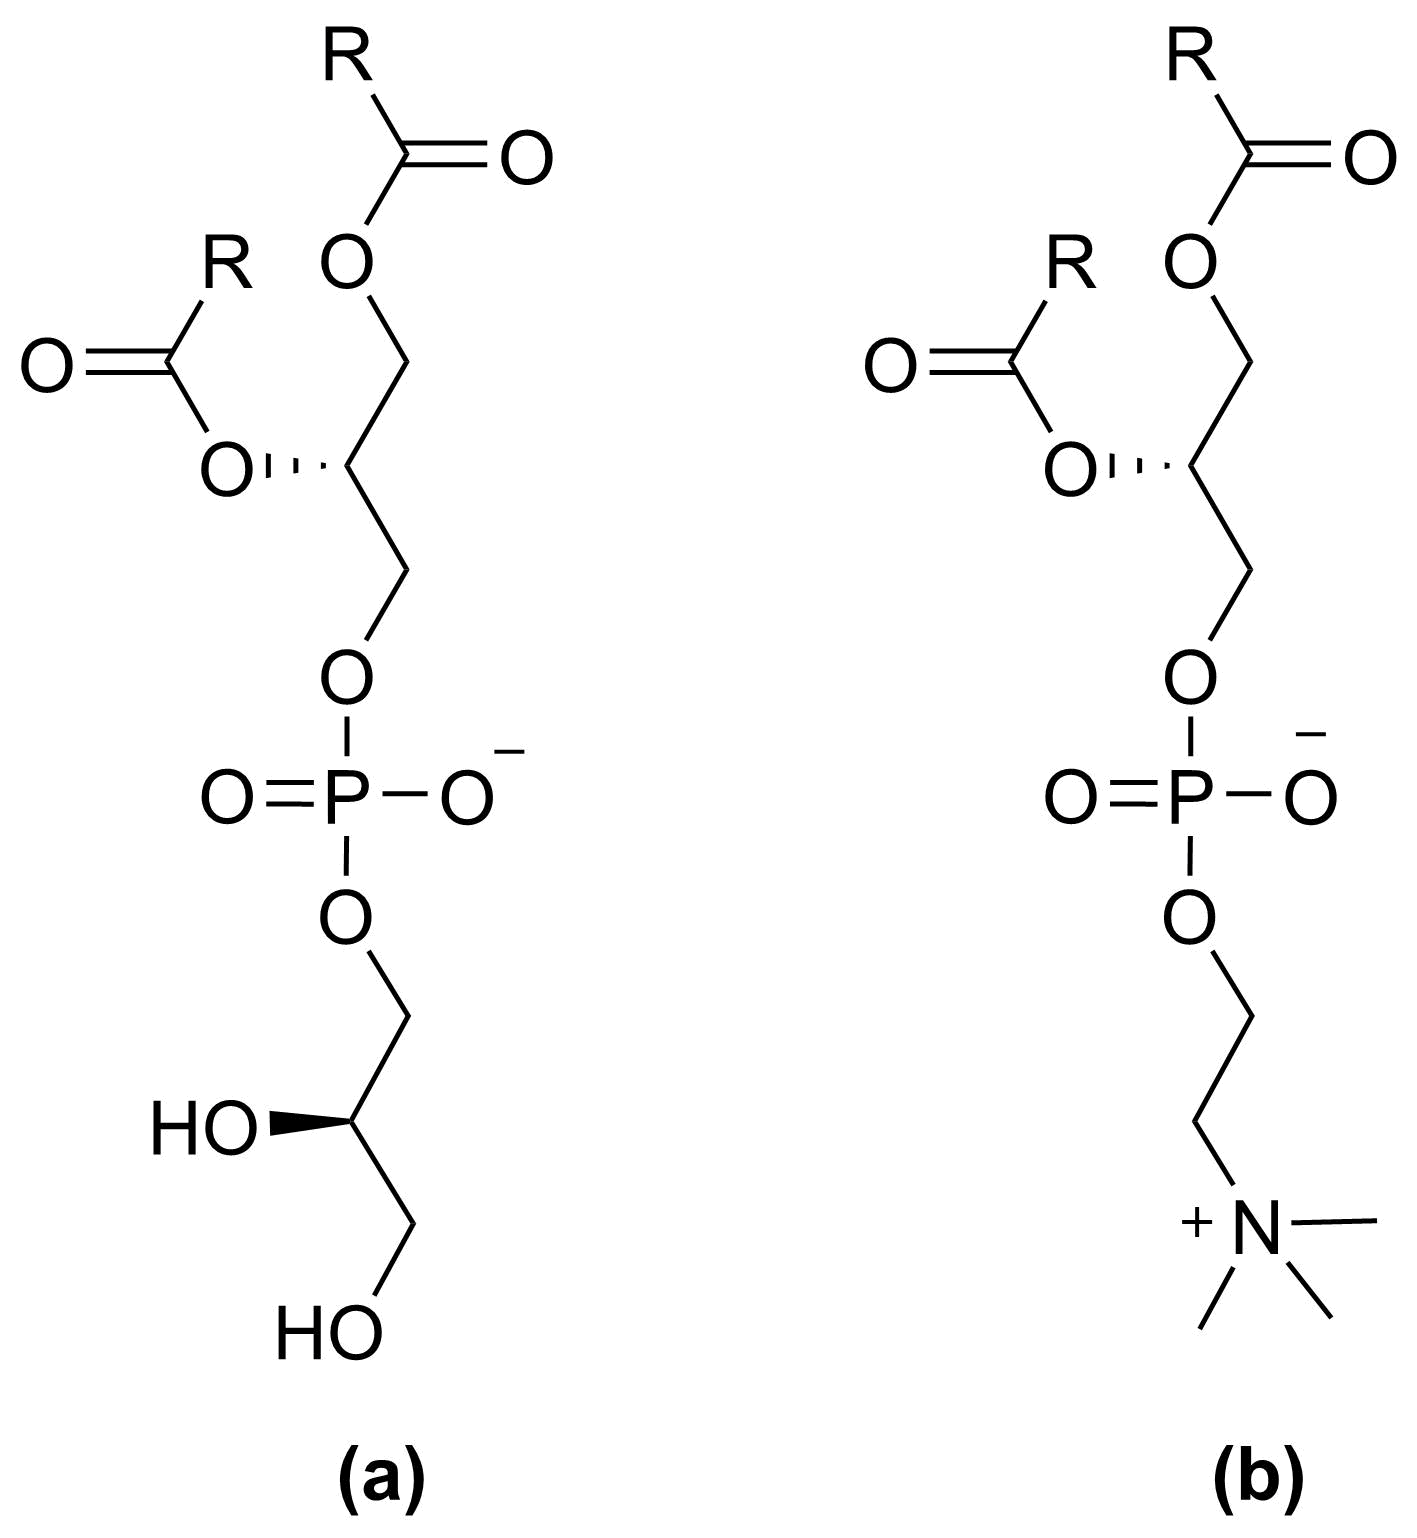
\includegraphics[width=\linewidth]{reflectometry1/head_groups}
    \caption{The two phospholipid forms investgated in this work, where R indicates the hydorcarbon tail; (a) phosphatidylglycerol (PG), (b) phosphocholine (PC).}
    \label{fig:heads}
\end{marginfigure}
%
Choline chloride (\SI{99}{\percent}, Sigma-Aldrich), glycerol (\SI{99}{\percent}, Sigma-Aldrich), d$_{9}$-choline chloride (\SI{99}{\percent}, \SI{98}{\percent} D, CK Isotopes), and d$_{8}$-glycerol (\SI{99}{\percent}, \SI{98}{\percent} D, CK Isotopes) were used in the preparation of the DES.
This is achieved by mixing a $1$:$2$ ratio of choline-chloride and glycerol and heating at \SI{80}{\celsius} until a homogeneous, transparent liquid is formed.\autocite{smith_deep_2014}
This was then stored under a dry atmosphere to reduce the amount of water dissolved in the solvent.

The limited availability of deuterated precursors lead to only a fully protonated and a partially deuterated\footnote{Abbreviated to hDES and hdDES respectively.} being prepared and used in the NR measurements.
The partially deuterated subphase was prepared using the following mixtures of precursors: \SI{1}{\mole} of \SI{0.38}{\mole} fraction of h-choline-chloride/\SI{0.62}{\mole} fraction of d-choline-chloride; and \SI{2}{\mole} of \SI{0.56}{\mole} fraction of h-glycerol/\SI{0.44}{\mole} fraction of d-glycerol.

The water content of the DES was assessed before and after each experiment by Karl-Fisher titration (Mettler Toledo DL32 Karl-Fischer Coulometer, Aqualine Electrolyte A, Aqualine Catholyte CG A) and found to be always below \SI{0.3}{wt/\percent}.
This was taken to be a negligible amount and would not have a considerable impact on the DES characteristics.\autocite{hammond_liquid_2016,hammond_resilience_2017}

1,2-dipalmitoyl-\emph{sn}-glycero-3-phosphocholine (C$_{16}$ tails, \SI{>99}{\percent}), 1,2-dimyristoyl-\emph{sn}-glycero-3-phosphocholine (C$_{14}$ tails, \SI{>99}{\percent}), and the sodium salt of 1,2-dimyristoyl-\emph{sn}-glycero-3-phospho-(1'-rac-glycerol) (C$_{14}$ tails, \SI{>99}{\percent})\footnote{Abbreviated to DPPC, DMPC, and DMPG respectively.} were obtained from Avanti Polar Lipids and 2-dilauroyl-\emph{sn}-glycero-3-phosphocholine (C$_{12}$ tails, \SI{>99}{\percent})\footnote{Abbreviated to DLPC.} was obtained from Sigma Aldrich and all were used without further purification.
Deuterated versions of DPPC (d$_{62}$-DPPC, \SI{>99}{\percent}, deuterated tails-only) and DMPC (d$_{54}$-DMPC, \SI{>99}{\percent}, deuterated tails-only) were obtained from Avanti Polar Lipids and used without further purification.
These phospholipids were dissolved in chloroform solution (\SI{0.5}{\milli\gram\per\milli\liter}) at room temperature.\footnote{PC indicates where the phospholipid molecule contains a phosphocholine head group, while PG indicates a phosphatidylglycerol head group, the chemical structures of these can be seen in Figure~\ref{fig:heads}.}

In the XRR experiment, the sample was prepared in-situ using the standard method for the spreading of insoluble monolayers on water.
A small amount of the phospholipid solution was spread on the liquid surface.
Following the evaporation of the chloroform, it is assumed that the resulting system is a subsurface of solvent with a monolayer of the phospholipid at the interface.
The surface concentration is then controlled by opening and closing the polytetrafluoroethylene\footnote{Abbreviated to PTFE} barriers of a Langmuir trough.
To reduce the volume used in the NR experiments, a small Delrin adsorption trough was used that did not have controllable PTFE barriers.
Therefore, although the surface concentration was nominally the same as for the XRR, the lack of precise control meant that it was determined to be inappropriate to co-refine the XRR and NR contrasts together.

\subsection{Methods}
The XRR measurements were carried out at the I07 beamline at the Diamond Light Source, with a photon energy of \SI{12.5}{\kilo\electronvolt} using the double-crystal deflector system.\autocite{arnold_implementation_2012}
The reflected intensity was measured for a $q$ range of \SIrange{0.018}{0.7}{\per\angstrom}.
The data were normalised with respect to the incident beam and the background was measured from off-specular reflection and subsequently subtracted.
All of the samples were allowed at least one hour to equilibrate and preserved under an argon atmosphere.
XRR data were collected for each of the phospholipids, DLPC, DMPC, DPPC, and DMPG at four SPs each,\footnote{DLPC: \SIlist{20;25;30;35}{\milli\newton\per\meter}, DMPC: \SIlist{20;25;30;40}{\milli\newton\per\meter}, DPPC: \SIlist{15;20;25;30}{\milli\newton\per\meter}, DMPG: \SIlist{15;20;25;30}{\milli\newton\per\meter}.} as measured with an aluminium Wilhelmy plate; measurements were conducted at \SIlist{7;22}{\celsius}.
An aluminium Wilhelmy plate was used over a traditional paper due to the low wettability of paper by the DES.

The NR experiments were performed on the FIGARO instrument at the Institut Laue-Langevin using time-of-flight methods.\autocite{campbell_figaro_2011}
Data were collected at two incident angles; \SIlist{0.62;3.8}{\degree}, providing a $q$ range from \SIrange{0.005}{0.18}{\per\angstrom}.
Two SPs for each phospholipid and contrast were measured.\footnote{DMPC: \SIlist{20;25}{\milli\newton\per\meter}, DPPC: \SIlist{15;20}{\milli\newton\per\meter}.}
As with the XRR measurements, the samples were given at least one hour to equilibrate, kept under an inert atmosphere.
All measurements were conducted at \SI{22}{\celsius}.
